\documentclass[10pt]{article}
\usepackage{graphicx}
\def\inputGnumericTable{}
\usepackage[latin1]{inputenc}
\usepackage{fullpage}
\usepackage{color}
\usepackage{array}
\usepackage{longtable}
\usepackage{calc}
\usepackage{multirow}
\usepackage{hhline}
\usepackage{ifthen}
\usepackage[none]{hyphenat}
\usepackage{graphicx}
\usepackage{listings}
\usepackage[english]{babel}
\usepackage{siunitx}
\usepackage{graphicx}
\usepackage{caption} 
\usepackage{booktabs}
\usepackage{array}
\usepackage{gensymb}
\usepackage{amssymb} % for \because
\usepackage{amsmath}   % for having text in math mode
\usepackage{extarrows} % for Row operations arrows
\usepackage{listings}
%\usepackage[utf8]{inputenc}
\lstset{
  frame=single,
  breaklines=true
}
\usepackage{hyperref}
\usepackage[margin=0.5in]{geometry}
  
%Following 2 lines were added to remove the blank page at the beginning
\usepackage{atbegshi}% http://ctan.org/pkg/atbegshi
\AtBeginDocument{\AtBeginShipoutNext{\AtBeginShipoutDiscard}}


%New macro definitions
\renewcommand{\labelenumi}{(\roman{enumi})}
\newcommand{\mydet}[1]{\ensuremath{\begin{vmatrix}#1\end{vmatrix}}}
\providecommand{\brak}[1]{\ensuremath{\left(#1\right)}}
\newcommand{\solution}{\noindent \textbf{Solution: }}
\newcommand{\myvec}[1]{\ensuremath{\begin{pmatrix}#1\end{pmatrix}}}
\providecommand{\norm}[1]{\left\lVert#1\right\rVert}
\providecommand{\abs}[1]{\left\vert#1\right\vert}
\let\vec\mathbf{}
\begin{document}

\begin{center}
\title{\textbf{CIRCLES}}
\date{\vspace{-5ex}} %Not to print date automatically
\maketitle
\end{center}
\section{9$^{th}$ Maths - Chapter 10}

This is Problem 2 from Exercise-10.6\\\\
Two chords AB and CD of lengths 5 cm and 11 cm respectively of a circle are parallel
to each other and are on opposite sides of its centre. If the distance between AB and
CD is 6 cm, find the radius of the circle.
\section{construction}
\begin{figure}[h!]
	\begin{center}
		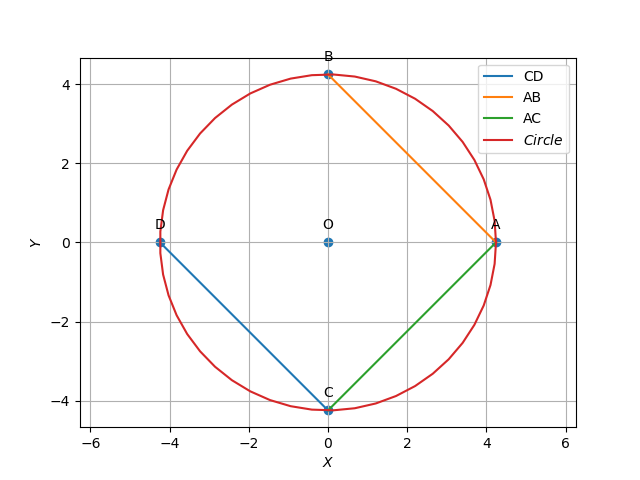
\includegraphics[width=5in]{./figs/fig.png}
	\end{center}
\caption{}
\label{fig:Fig1}
\end{figure}
The input parameters for this construction are\\
\begin{table}[h!]
	\centering
	%%%%%%%%%%%%%%%%%%%%%%%%%%%%%%%%%%%%%%%%%%%%%%%%%%%%%%%%%%%%%%%%%%%%%%
%%                                                                  %%
%%  This is the header of a LaTeX2e file exported from Gnumeric.    %%
%%                                                                  %%
%%  This file can be compiled as it stands or included in another   %%
%%  LaTeX document. The table is based on the longtable package so  %%
%%  the longtable options (headers, footers...) can be set in the   %%
%%  preamble section below (see PRAMBLE).                           %%
%%                                                                  %%
%%  To include the file in another, the following two lines must be %%
%%  in the including file:                                          %%
%%        \def\inputGnumericTable{}                                 %%
%%  at the beginning of the file and:                               %%
%%        \input{name-of-this-file.tex}                             %%
%%  where the table is to be placed. Note also that the including   %%
%%  file must use the following packages for the table to be        %%
%%  rendered correctly:                                             %%
%%    \usepackage[latin1]{inputenc}                                 %%
%%    \usepackage{color}                                            %%
%%    \usepackage{array}                                            %%
%%    \usepackage{longtable}                                        %%
%%    \usepackage{calc}                                             %%
%%    \usepackage{multirow}                                         %%
%%    \usepackage{hhline}                                           %%
%%    \usepackage{ifthen}                                           %%
%%  optionally (for landscape tables embedded in another document): %%
%%    \usepackage{lscape}                                           %%
%%                                                                  %%
%%%%%%%%%%%%%%%%%%%%%%%%%%%%%%%%%%%%%%%%%%%%%%%%%%%%%%%%%%%%%%%%%%%%%%



%%  This section checks if we are begin input into another file or  %%
%%  the file will be compiled alone. First use a macro taken from   %%
%%  the TeXbook ex 7.7 (suggestion of Han-Wen Nienhuys).            %%
\def\ifundefined#1{\expandafter\ifx\csname#1\endcsname\relax}


%%  Check for the \def token for inputed files. If it is not        %%
%%  defined, the file will be processed as a standalone and the     %%
%%  preamble will be used.                                          %%
\ifundefined{inputGnumericTable}

%%  We must be able to close or not the document at the end.        %%
	\def\gnumericTableEnd{\end{document}}


%%%%%%%%%%%%%%%%%%%%%%%%%%%%%%%%%%%%%%%%%%%%%%%%%%%%%%%%%%%%%%%%%%%%%%
%%                                                                  %%
%%  This is the PREAMBLE. Change these values to get the right      %%
%%  paper size and other niceties.                                  %%
%%                                                                  %%
%%%%%%%%%%%%%%%%%%%%%%%%%%%%%%%%%%%%%%%%%%%%%%%%%%%%%%%%%%%%%%%%%%%%%%

	\documentclass[12pt%
			  %,landscape%
                    ]{report}
       \usepackage[latin1]{inputenc}
       \usepackage{fullpage}
       \usepackage{color}
       \usepackage{array}
       \usepackage{longtable}
       \usepackage{calc}
       \usepackage{multirow}
       \usepackage{hhline}
       \usepackage{ifthen}

	\begin{document}


%%  End of the preamble for the standalone. The next section is for %%
%%  documents which are included into other LaTeX2e files.          %%
\else

%%  We are not a stand alone document. For a regular table, we will %%
%%  have no preamble and only define the closing to mean nothing.   %%
    \def\gnumericTableEnd{}

%%  If we want landscape mode in an embedded document, comment out  %%
%%  the line above and uncomment the two below. The table will      %%
%%  begin on a new page and run in landscape mode.                  %%
%       \def\gnumericTableEnd{\end{landscape}}
%       \begin{landscape}


%%  End of the else clause for this file being \input.              %%
\fi

%%%%%%%%%%%%%%%%%%%%%%%%%%%%%%%%%%%%%%%%%%%%%%%%%%%%%%%%%%%%%%%%%%%%%%
%%                                                                  %%
%%  The rest is the gnumeric table, except for the closing          %%
%%  statement. Changes below will alter the table's appearance.     %%
%%                                                                  %%
%%%%%%%%%%%%%%%%%%%%%%%%%%%%%%%%%%%%%%%%%%%%%%%%%%%%%%%%%%%%%%%%%%%%%%

\providecommand{\gnumericmathit}[1]{#1} 
%%  Uncomment the next line if you would like your numbers to be in %%
%%  italics if they are italizised in the gnumeric table.           %%
%\renewcommand{\gnumericmathit}[1]{\mathit{#1}}
\providecommand{\gnumericPB}[1]%
{\let\gnumericTemp=\\#1\let\\=\gnumericTemp\hspace{0pt}}
 \ifundefined{gnumericTableWidthDefined}
        \newlength{\gnumericTableWidth}
        \newlength{\gnumericTableWidthComplete}
        \newlength{\gnumericMultiRowLength}
        \global\def\gnumericTableWidthDefined{}
 \fi
%% The following setting protects this code from babel shorthands.  %%
 \ifthenelse{\isundefined{\languageshorthands}}{}{\languageshorthands{english}}
%%  The default table format retains the relative column widths of  %%
%%  gnumeric. They can easily be changed to c, r or l. In that case %%
%%  you may want to comment out the next line and uncomment the one %%
%%  thereafter                                                      %%
\providecommand\gnumbox{\makebox[0pt]}
%%\providecommand\gnumbox[1][]{\makebox}

%% to adjust positions in multirow situations                       %%
\setlength{\bigstrutjot}{\jot}
\setlength{\extrarowheight}{\doublerulesep}

%%  The \setlongtables command keeps column widths the same across  %%
%%  pages. Simply comment out next line for varying column widths.  %%
\setlongtables

\setlength\gnumericTableWidth{%
	53pt+%
	53pt+%
	94pt+%
	53pt+%
0pt}
\def\gumericNumCols{4}
\setlength\gnumericTableWidthComplete{\gnumericTableWidth+%
         \tabcolsep*\gumericNumCols*2+\arrayrulewidth*\gumericNumCols}
\ifthenelse{\lengthtest{\gnumericTableWidthComplete > \linewidth}}%
         {\def\gnumericScale{1*\ratio{\linewidth-%
                        \tabcolsep*\gumericNumCols*2-%
                        \arrayrulewidth*\gumericNumCols}%
{\gnumericTableWidth}}}%
{\def\gnumericScale{1}}

%%%%%%%%%%%%%%%%%%%%%%%%%%%%%%%%%%%%%%%%%%%%%%%%%%%%%%%%%%%%%%%%%%%%%%
%%                                                                  %%
%% The following are the widths of the various columns. We are      %%
%% defining them here because then they are easier to change.       %%
%% Depending on the cell formats we may use them more than once.    %%
%%                                                                  %%
%%%%%%%%%%%%%%%%%%%%%%%%%%%%%%%%%%%%%%%%%%%%%%%%%%%%%%%%%%%%%%%%%%%%%%

\ifthenelse{\isundefined{\gnumericColA}}{\newlength{\gnumericColA}}{}\settowidth{\gnumericColA}{\begin{tabular}{@{}p{53pt*\gnumericScale}@{}}x\end{tabular}}
\ifthenelse{\isundefined{\gnumericColB}}{\newlength{\gnumericColB}}{}\settowidth{\gnumericColB}{\begin{tabular}{@{}p{53pt*\gnumericScale}@{}}x\end{tabular}}
\ifthenelse{\isundefined{\gnumericColC}}{\newlength{\gnumericColC}}{}\settowidth{\gnumericColC}{\begin{tabular}{@{}p{83pt*\gnumericScale}@{}}x\end{tabular}}
\ifthenelse{\isundefined{\gnumericColD}}{\newlength{\gnumericColD}}{}\settowidth{\gnumericColD}{\begin{tabular}{@{}p{53pt*\gnumericScale}@{}}x\end{tabular}}

	\begin{center}
\begin{tabular}[c]{%
	b{\gnumericColA}%
	b{\gnumericColB}%
	b{\gnumericColC}%
	b{\gnumericColD}%
	}

%%%%%%%%%%%%%%%%%%%%%%%%%%%%%%%%%%%%%%%%%%%%%%%%%%%%%%%%%%%%%%%%%%%%%%
%%  The longtable options. (Caption, headers... see Goosens, p.124) %%
%	\caption{The Table Caption.}             \\	%
% \hline	% Across the top of the table.
%%  The rest of these options are table rows which are placed on    %%
%%  the first, last or every page. Use \multicolumn if you want.    %%

%%  Header for the first page.                                      %%
%	\multicolumn{4}{c}{The First Header} \\ \hline 
%	\multicolumn{1}{c}{colTag}	%Column 1
%	&\multicolumn{1}{c}{colTag}	%Column 2
%	&\multicolumn{1}{c}{colTag}	%Column 3
%	&\multicolumn{1}{c}{colTag}	\\ \hline %Last column
%	\endfirsthead

%%  The running header definition.                                  %%
%	\hline
%	\multicolumn{4}{l}{\ldots\small\slshape continued} \\ \hline
%	\multicolumn{1}{c}{colTag}	%Column 1
%	&\multicolumn{1}{c}{colTag}	%Column 2
%	&\multicolumn{1}{c}{colTag}	%Column 3
%	&\multicolumn{1}{c}{colTag}	\\ \hline %Last column
%	\endhead

%%  The running footer definition.                                  %%
%	\hline
%	\multicolumn{4}{r}{\small\slshape continued\ldots} \\
%	\endfoot

%%  The ending footer definition.                                   %%
%	\multicolumn{4}{c}{That's all folks} \\ \hline 
%	\endlastfoot
%%%%%%%%%%%%%%%%%%%%%%%%%%%%%%%%%%%%%%%%%%%%%%%%%%%%%%%%%%%%%%%%%%%%%%

\hhline{|-|-|-~}
  \multicolumn{1}{|p{\gnumericColA}|}%
 {\gnumericPB{\centering}\gnumbox{\textbf{Symbol}}}
 &\multicolumn{1}{p{\gnumericColB}|}%
 {\gnumericPB{\centering}\gnumbox{\textbf{Value}}}
 &\multicolumn{1}{p{\gnumericColC}|}%
 {\gnumericPB{\centering}\gnumbox{\textbf{Description}}}
 &
\\
\hhline{|---|~}
  \multicolumn{1}{|p{\gnumericColA}|}%
 {\gnumericPB{\centering}\gnumbox{$\theta$}}
 &\multicolumn{1}{p{\gnumericColB}|}%
 {\gnumericPB{\centering}\gnumbox{$0\degree$}}
 &\multicolumn{1}{p{\gnumericColC}|}%
 {\gnumericPB{\centering}\gnumbox{assumed angle}}
 &
\\
\hhline{|---|~}
  \multicolumn{1}{|p{\gnumericColA}|}%
 {\gnumericPB{\centering}\gnumbox{$\phi$}}
 &\multicolumn{1}{p{\gnumericColB}|}%
 {\gnumericPB{\centering}\gnumbox{$90\degree$}}
 &\multicolumn{1}{p{\gnumericColC}|}%
 {\gnumericPB{\centering}\gnumbox{assumed angle}}
 &
\\
\hhline{|---|~}
  \multicolumn{1}{|p{\gnumericColA}|}%
 {\gnumericPB{\centering}\gnumbox{$\vec{A}$}}
 &\multicolumn{1}{p{\gnumericColB}|}%
 {\gnumericPB{\centering}\gnumbox{$\myvec{1\\0}$}}
 &\multicolumn{1}{p{\gnumericColC}|}%
 {\gnumericPB{\centering}\gnumbox{point A}}
 &
\\
\hhline{|---|~}
  \multicolumn{1}{|p{\gnumericColA}|}%
 {\gnumericPB{\centering}\gnumbox{$\vec{B}$}}
 &\multicolumn{1}{p{\gnumericColB}|}%
 {\gnumericPB{\centering}\gnumbox{$\myvec{0\\1}$}}
 &\multicolumn{1}{p{\gnumericColC}|}%
 {\gnumericPB{\centering}\gnumbox{point B}}
 &
\\
\hhline{|---|~}
  \multicolumn{1}{|p{\gnumericColA}|}%
 {\gnumericPB{\centering}\gnumbox{$\vec{m}$}}
 &\multicolumn{1}{p{\gnumericColB}|}%
 {\gnumericPB{\centering}\gnumbox{$\myvec{-1\\1}$}}
 &\multicolumn{1}{p{\gnumericColC}|}%
 {\gnumericPB{\centering}\gnumbox{directional vector}}
 &
\\
\hhline{|---|~}
  \multicolumn{1}{|p{\gnumericColA}|}%
 {\gnumericPB{\centering}\gnumbox{$\vec{n}$}}
 &\multicolumn{1}{p{\gnumericColB}|}%
 {\gnumericPB{\centering}\gnumbox{$\myvec{1\\1}$}}
 &\multicolumn{1}{p{\gnumericColC}|}%
 {\gnumericPB{\centering}\gnumbox{normal vector}}
 &
\\
\hhline{|-|-|-|~}
\end{tabular}
 \end{center}

\ifthenelse{\isundefined{\languageshorthands}}{}{\languageshorthands{\languagename}}
\gnumericTableEnd

\label{table:1}
\end{table}\\
\begin{align}
\vec{A}=r\myvec{\cos{\theta_1}\\\sin{\theta_1}},\vec{B}=r\myvec{\cos{\theta_2}\\\sin{\theta_2}},\vec{C}=r\myvec{\cos{\theta_3}\\\sin{\theta_3}},\vec{D}=r\myvec{\cos{\theta_4}\\\sin{\theta_4}}
\end{align}
\solution
Lines AB and CD are parallel.\\
Therefore,\\
\begin{align}
\vec{m_1}=&\vec{m_2}\\
\myvec{\cos{\theta_1}-\cos{\theta_2}\\\sin{\theta_1}-\sin{\theta_2}}=&\myvec{\cos{\theta_3}-\cos{\theta_4}\\\sin{\theta_3}-\sin{\theta_4}}\\
\implies\myvec{1\\-1}=&\myvec{1\\-1}
\label{eq:1}
\end{align}
from \eqref{eq:1} the normal vector is given by
\begin{align}
\vec{n}=\myvec{-1\\-1}
\end{align}
The line equation of AB is 
\begin{align}
r\myvec{-1&-1}\vec{x}=&r^2\myvec{-1&-1}\myvec{1\\0}\\
\myvec{-1&-1}=&-r
\label{eq:2}
\end{align}
The line equation of CD is 
\begin{align}
r\myvec{-1&-1}\vec{x}=&r^2\myvec{-1&-1}\myvec{0\\-1}\\
\myvec{-1&-1}=&r
\label{eq:3}
\end{align}
from \eqref{eq:2} and \eqref{eq:3}
\begin{align}
c_1=-r,c_2=r
\end{align}
The distance between parallel lines is
\begin{align}
d=&\frac{\abs{c_1-c_2}}{\norm{\vec{n}}}\\
\implies 6=&\frac{2r}{\sqrt{2}}\\
\implies r=&4.24
\end{align}
\end{document}
